\documentclass[conference]{IEEEtran}
\IEEEoverridecommandlockouts
\usepackage[utf8]{inputenc}
\usepackage[T1]{fontenc}
\usepackage{graphicx}
\usepackage{booktabs}
\usepackage{amsmath}
\usepackage{siunitx}
\usepackage{xcolor}
\usepackage{url}
\usepackage[hidelinks]{hyperref}
\usepackage{cite}
\sisetup{group-separator={,}, detect-all}
\graphicspath{{figures/}}

\begin{document}

\title{Market Structure of the Best-Selling Nintendo Switch Games:\\
An Exploratory Data Analysis in Python}

\author{\IEEEauthorblockN{David Zuluaga Henao}
\IEEEauthorblockA{\textit{School of Applied Sciences and Engineering} \\
\textit{Universidad EAFIT}, Medellín, Colombia \\
Programming Fundamentals, 2022-1}}

\maketitle

\begin{abstract}
This report analyzes the 43 Nintendo Switch games that had sold more than one million copies by early 2021, which add up to 292.2 million copies. Using Python (pandas, NumPy, Matplotlib and SciPy), the data were cleaned, grouped by genre, developer and publisher, and used to test four hypotheses from the course proposal. Nintendo EPD developed 14 of the titles and accounts for 55.5\,\% of all copies sold, 13.3 times the mean per developer (supported). Platformer is the best-selling genre (18.0\,\%) and also the genre with the most titles (7). The claim that role-playing has the most titles holds only if action and tactical role-playing games are counted together (9 titles), so this hypothesis is partly supported. First- and second-party publishers (Nintendo and The Pokémon Company) hold 79.1\,\% of the titles and 93.7\,\% of the sales (supported). Sales are strongly right-skewed: only 14 titles (32.6\,\%) sell more than the mean of 6.80 million, so the hypothesis that most titles sell above the mean is rejected. This version fixes several processing errors in the original deliverable. The fixes change the mean sales per developer and the third-party share.
\end{abstract}

\begin{IEEEkeywords}
exploratory data analysis, pandas, video game sales, Nintendo Switch, hypothesis testing, data visualization
\end{IEEEkeywords}

\section{Introduction}
The Nintendo Switch is a hybrid console released in March 2017. Its catalog makes it possible to ask which companies and genres drive commercial success on a single platform. This project applies the tools of the Programming Fundamentals course (data structures, functions, loops, conditionals and the NumPy, pandas and Matplotlib libraries) to a public dataset of the console's best-selling games. The goals are to:
\begin{enumerate}
  \item describe how sales are distributed by genre, developer and publisher;
  \item test four hypotheses stated in the project proposal; and
  \item deliver a reproducible script that writes every table and figure and shows them in a graphical interface.
\end{enumerate}

The results are relevant for market analysis. They show how strongly the console's commercial success depends on its platform holder, and which genres turn into the most sales.

\section{Dataset}
The data come from the Kaggle dataset \emph{Top Selling Switch Games}~\cite{kaggle}, which reproduces the Wikipedia list of best-selling Switch games~\cite{wiki}. It has 43 rows, one per game with at least one million copies sold, and the eight columns in Table~\ref{tab:vars}.

\begin{table}[!t]
\caption{Variables of the dataset}
\label{tab:vars}
\centering
\footnotesize
\begin{tabular}{@{}lll@{}}
\toprule
Column & Type & Description \\
\midrule
No. & integer & Rank in the source list \\
Title & text & Game title \\
Copies sold & float & Units sold, in millions \\
As of & date & Date of the sales figure \\
Release date & date & First release date \\
Genre(s) & category & Main genre (22 values) \\
Developer(s) & category & Developer studio (25 values) \\
Publisher(s) & category & Publisher (12 values) \\
\bottomrule
\end{tabular}
\end{table}

Three limitations shape the interpretation:
\begin{enumerate}
  \item The list is \emph{truncated} at one million copies, so it describes the best-sellers and not the whole catalog.
  \item The ``As of'' dates range from March 2018 to February 2021, so the sales figures are not a single snapshot.
  \item For seven games the publisher field keeps only one regional publisher (e.g., ``JP: Koei Tecmo''), even when another company published the game elsewhere.
\end{enumerate}

\section{Hypotheses}
The proposal stated four hypotheses:
\begin{itemize}
  \item \textbf{H1:} Nintendo EPD is the developer with the most sales among the best-sellers and is above the mean sales per developer.
  \item \textbf{H2:} Platformer is the genre with the largest share of sales, and role-playing is the genre with the most successful titles.
  \item \textbf{H3:} Third-party companies have far fewer best-selling titles than first- and second-party companies, because Nintendo publishes more titles for the console.
  \item \textbf{H4:} Most titles sell more than the mean sales of the list.
\end{itemize}

H2 and H4 are descriptive. H1 and H3 were proposed as causal (``and therefore'', ``because''). With observational sales data, however, only the association can be tested, not the cause. Glossary~\cite{otaku}:
\begin{itemize}
  \item A \emph{first-party} developer belongs to the console manufacturer.
  \item A \emph{second-party} developer is an external studio that makes exclusive games published by the manufacturer.
  \item A \emph{third-party} company makes games for any platform.
\end{itemize}
As in the original work, first- and second-party games are analyzed as one group.

\section{Methodology}

\subsection{Tools and workflow}
The analysis is a single script, \texttt{switch\_sales\_analysis.py} (Python~3.10 or later) built on pandas~\cite{pandas}, NumPy~\cite{numpy}, Matplotlib~\cite{mpl} and SciPy~\cite{scipy}. It:
\begin{enumerate}
  \item loads and cleans the CSV file with pandas;
  \item builds grouped tables with \texttt{groupby};
  \item evaluates the hypotheses;
  \item saves six CSV tables, a JSON summary and ten PNG figures; and
  \item opens a Tkinter window with the hypotheses, the tables, the full dataset and an interactive viewer for the figures (Fig.~\ref{fig:gui}).
\end{enumerate}
If a library is missing, the script creates a local virtual environment and installs it automatically, so it runs with a single click.

\subsection{Data cleaning and derived variables}
\begin{itemize}
  \item Dates were parsed with the format \texttt{\%d-\%b-\%y}.
  \item The developers ``Nintendo'' (\emph{Super Mario 3D All-Stars}) and ``Nintendo EPD'' were merged into one studio group, which leaves 24 developers.
  \item Regional prefixes (``JP:'', ``NA/PAL:'') were removed from the publisher and recorded in a flag. This merges ``JP: The Pokémon Company'' with ``The Pokémon Company'' and leaves 11 publishers.
  \item Each game was assigned to the \emph{first/second party} group if its publisher is Nintendo or The Pokémon Company (co-owned by Nintendo); all other games are \emph{third party}.
  \item The time on the market is the number of years between the release date and the ``As of'' date. The role-playing family (role-playing, action RPG and tactical RPG) was added as a sensitivity grouping for H2.
\end{itemize}

\subsection{Corrections to the original deliverable}
\begin{itemize}
  \item The total sales were truncated with \texttt{int()} (292 instead of 292.2 million) before the means were computed.
  \item Nintendo and Nintendo EPD were counted as two developers, so the mean per developer was $292/25 = 11.68$~M. It is now $292.2/24 = 12.18$~M.
  \item The three games published by The Pokémon Company were classified as third party, which gave 27.9\,\% third-party titles instead of 20.9\,\%.
  \item Pie charts with 22 slices were replaced by sorted bar charts, and the developer bar chart now shows its reference lines.
\end{itemize}

\subsection{Statistics}
\begin{itemize}
  \item \textbf{Descriptive statistics:} counts, sums, means, medians and sample skewness.
  \item \textbf{H3:} the one-sided Mann--Whitney $U$ test~\cite{mw} compares the sales per title of the two groups. It does not assume normality, which suits the skewed sales data.
  \item \textbf{Time on the market:} its association with sales is measured with Spearman's rank correlation $\rho$.
  \item \textbf{Significance level:} $\alpha = 0.05$ for all tests.
\end{itemize}

\section{Results}

\subsection{Overall distribution}
Sales per title have a mean of 6.80~M and a median of 2.87~M, with a standard deviation of 8.36~M and a skewness of 1.78 (Fig.~\ref{fig:dist}). Sales are highly concentrated (Fig.~\ref{fig:pareto}):
\begin{itemize}
  \item the top five titles account for 44.2\,\% of all copies;
  \item the top ten, for 67.8\,\%;
  \item the top twenty, for 86.0\,\%.
\end{itemize}
Every one of the top 15 games is a first/second-party title (Fig.~\ref{fig:top}). The best-selling game is \emph{Mario Kart~8 Deluxe}, with 33.41~M copies.

\begin{figure}[!htb]
\centering

\includegraphics[width=0.95\columnwidth]{01_top_titles.png}
\caption{Top 20 best-selling Nintendo Switch games, colored by publisher group.}
\label{fig:top}
\end{figure}

\begin{figure}[!htb]
\centering

\includegraphics[width=\columnwidth]{08_title_distribution.png}
\caption{Distribution of copies sold per title. Only 14 of the 43 titles are above the mean.}
\label{fig:dist}
\end{figure}

\subsection{Genres}
Table~\ref{tab:genres} and Fig.~\ref{fig:genres} summarize the 22 genres. Platformer leads in both sales (52.70~M, 18.0\,\%) and number of titles (7). The single social-simulation title, \emph{Animal Crossing: New Horizons}, sells more than most genres combined. The mean sales per genre is 13.28~M, and only seven genres are above it.

\begin{table}[!t]
\caption{Top genres by copies sold}
\label{tab:genres}
\centering
\footnotesize
\begin{tabular}{@{}lrrr@{}}
\toprule
Genre & Titles & Sales (M) & Share (\%) \\
\midrule
Platformer & 7 & 52.70 & 18.0 \\
Role-playing & 4 & 38.40 & 13.1 \\
Action-adventure & 4 & 36.04 & 12.3 \\
Kart racing & 2 & 34.49 & 11.8 \\
Social simulation & 1 & 31.18 & 10.7 \\
Fighting & 3 & 26.39 & 9.0 \\
Party & 3 & 20.20 & 6.9 \\
Other 15 genres & 19 & 52.80 & 18.1 \\
\midrule
RPG family (3 sub-genres) & 9 & 47.75 & 16.3 \\
\bottomrule
\end{tabular}
\end{table}

\begin{figure*}[!t]
\centering

\includegraphics[width=0.72\textwidth]{02_genres.png}
\caption{Sales (left) and number of titles (right) by genre. The two genres named in H2 are highlighted.}
\label{fig:genres}
\end{figure*}

\subsection{Developers}
The 43 titles come from 24 developers. Nintendo EPD made 14 of them and sold 162.15~M copies (55.5\,\%), almost five times the second developer, Game Freak (33.35~M in two Pokémon titles). Only four developers are above the mean of 12.18~M (Fig.~\ref{fig:devs}): Nintendo EPD, Game Freak, Bandai Namco Studios (25.01~M) and NDcube (16.44~M). The median developer sold just 2.79~M, and 20 of the 24 developers sold less than 10~M copies in total.

\begin{figure}[!htb]
\centering

\includegraphics[width=0.92\columnwidth]{04_developers.png}
\caption{Total copies sold by developer, with the mean and median per developer.}
\label{fig:devs}
\end{figure}

\subsection{Publishers and first/second vs third party}
Nintendo published 31 titles (239.25~M copies, 81.9\,\%) and The Pokémon Company three (34.51~M). The other nine publishers have one title each.

Together, the first/second-party group holds 34 titles (79.1\,\%) and 273.76~M copies (93.7\,\%), as summarized in Table~\ref{tab:eco} and Fig.~\ref{fig:eco}. The best third-party title, \emph{Hyrule Warriors: Age of Calamity}, is a Zelda spin-off developed by Omega Force. Its 3.50~M copies would not place it in the top 15.

The median sales per title are 3.05~M for the first/second-party group and 2.00~M for third parties. The Mann--Whitney test gives $U = 223$ and one-sided $p = 0.019$, so first/second-party titles also tend to sell more per title.

\begin{table}[!t]
\caption{First/second-party vs third-party titles}
\label{tab:eco}
\centering
\footnotesize
\begin{tabular}{@{}lrrrr@{}}
\toprule
Group & Titles & Sales (M) & Share (\%) & Median (M) \\
\midrule
First/second party & 34 & 273.76 & 93.7 & 3.05 \\
Third party & 9 & 18.44 & 6.3 & 2.00 \\
\bottomrule
\end{tabular}
\end{table}

\begin{figure*}[!t]
\centering

\includegraphics[width=0.7\textwidth]{07_ecosystem.png}
\caption{Share of titles and sales (left) and sales per title (right, log scale) for first/second-party and third-party games. Black lines mark the medians.}
\label{fig:eco}
\end{figure*}

\subsection{Time on the market}
Games that had been on sale longer tend to have higher figures (Fig.~\ref{fig:time}): Spearman $\rho = 0.34$, $p = 0.028$. The effect is moderate. \emph{Animal Crossing: New Horizons} reached 31.18~M copies in only nine months, while several 2017 titles stayed below 3~M. Because the figures were taken on different dates, rankings of recent titles understate their long-term sales.

\begin{figure}[!htb]
\centering

\includegraphics[width=\columnwidth]{09_pareto.png}
\caption{Cumulative share of total sales by number of titles (Pareto curve).}
\label{fig:pareto}
\end{figure}

\begin{figure}[!htb]
\centering

\includegraphics[width=\columnwidth]{10_time_on_market.png}
\caption{Copies sold vs years between release and the sales figure (log scale).}
\label{fig:time}
\end{figure}

\section{Hypothesis Evaluation}
Table~\ref{tab:hyp} summarizes the evaluation of the four hypotheses.

\begin{table}[!t]
\caption{Evaluation of the hypotheses}
\label{tab:hyp}
\centering
\footnotesize
\begin{tabular}{@{}p{0.06\columnwidth}p{0.2\columnwidth}p{0.6\columnwidth}@{}}
\toprule
& Result & Evidence \\
\midrule
H1 & Supported & Nintendo EPD: 162.15~M copies (55.5\,\%), 13.3 $\times$ the developer mean of 12.18~M. \\
H2 & Partly supported & Platformer leads sales (18.0\,\%) and titles (7). ``Role-playing'' has 4 titles; the RPG family has 9. \\
H3 & Supported & 79.1\,\% of titles and 93.7\,\% of sales are first/second party; $p = 0.019$ for higher sales per title. \\
H4 & Rejected & 14 of 43 titles (32.6\,\%) are above the mean of 6.80~M; the median is 2.87~M. \\
\bottomrule
\end{tabular}
\end{table}

\textbf{H1} is supported: Nintendo EPD is by far the top developer. However, a descriptive analysis cannot confirm the causal wording (``most popular, and therefore''). Nintendo EPD also develops the console's flagship franchises, which is a confounding factor.

\textbf{H2} depends on how the genres are labeled. The first part is correct. The second part is false for the exact label but true for the role-playing family, which also sells 47.75~M copies, close to platformers.

\textbf{H3} is supported both in number of titles and in sales. The one-million-copy cutoff removes most third-party releases from the list, so the gap in the full catalog cannot be measured with these data.

\textbf{H4} is rejected. With a skewed distribution, the mean is pulled up by a few hits: the four titles above 21~M copies alone hold 37.3\,\% of all sales. The median is a better description of a typical best-seller.

\section{Discussion and Limitations}
The Switch best-seller market is dominated by the platform holder's own franchises. Nintendo franchises (Mario, Zelda, Pokémon, Animal Crossing, Smash Bros.\ and Splatoon) account for all of the top ten titles. For third parties, success on the console appears to come from licensed spin-offs (\emph{Hyrule Warriors}) or cross-platform hits (\emph{Among Us}, \emph{Minecraft}), and it stays in the 1--3.5~M range.

The limitations of the analysis are:
\begin{itemize}
  \item the one-million-copy cutoff;
  \item sales figures taken on different dates;
  \item a single genre per game; and
  \item publisher information that is incomplete for regional releases.
\end{itemize}
A future version could use a full sales database, normalize sales by months on the market, and add review scores or prices as explanatory variables.

\section{Conclusions}
\begin{itemize}
  \item Nintendo EPD is the dominant developer, with 14 titles and 55.5\,\% of all copies sold among the best-sellers (H1 supported).
  \item Platformer is the leading genre in both sales and titles. Role-playing leads in titles only if its sub-genres are grouped (H2 partly supported).
  \item First- and second-party publishers hold 79.1\,\% of the titles and 93.7\,\% of the sales, and their games sell more per title (H3 supported).
  \item Sales are strongly concentrated: two thirds of the titles are below the mean, and the ten best-sellers hold 67.8\,\% of the copies (H4 rejected).
  \item Correcting the data processing (exact sums, merged developer names, publisher cleaning) changed the mean per developer from 11.68~M to 12.18~M and the third-party share of titles from 27.9\,\% to 20.9\,\%. This shows how small coding decisions affect the conclusions of a data analysis.
\end{itemize}

\appendix[Reproducibility]
Run \texttt{python 02\_Analysis/switch\_sales\_analysis.py} (or double-click \texttt{run\_analysis.bat} on Windows). The script installs its dependencies on the first run, prints the results, saves the outputs to \texttt{02\_Analysis/results} and \texttt{02\_Analysis/figures}, and opens the interface in Fig.~\ref{fig:gui}.

\begin{figure}[!htb]
\centering
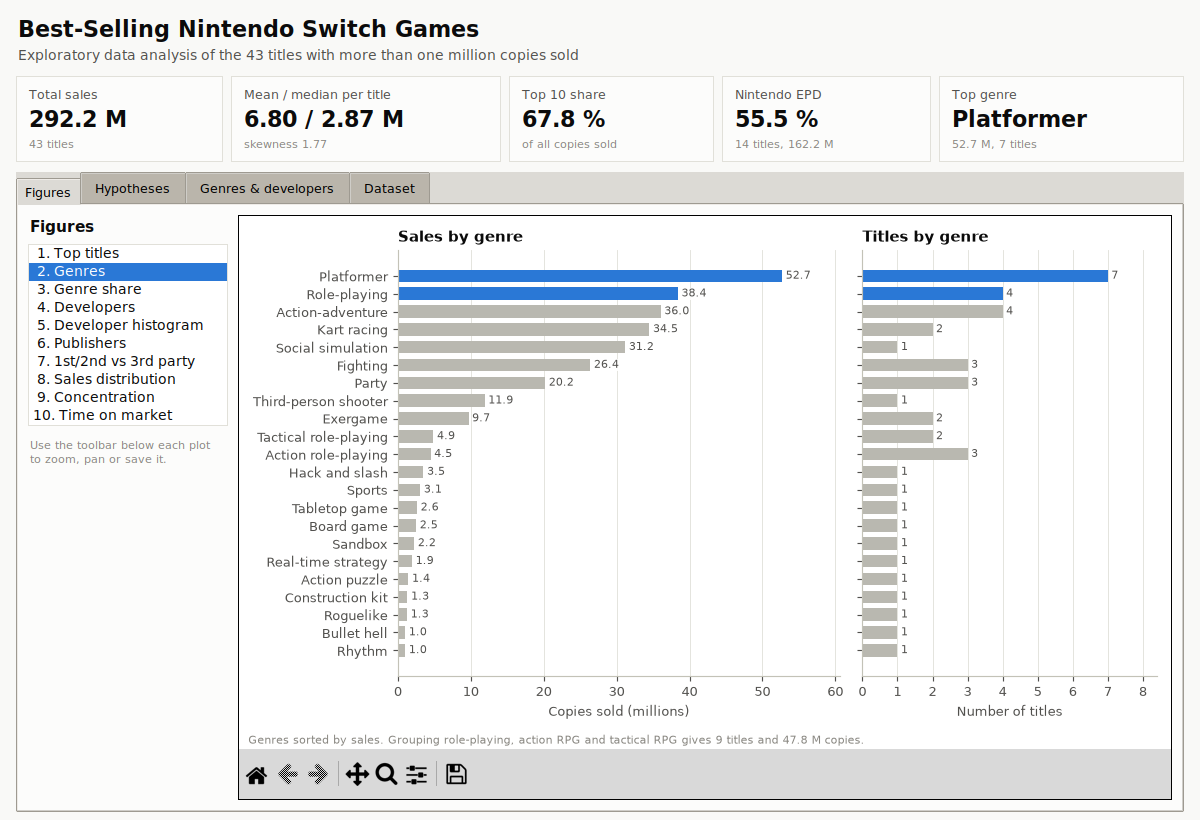
\includegraphics[width=\columnwidth]{gui_figures.png}
\caption{Graphical interface: summary tiles, hypothesis tab, tables, dataset viewer and interactive figure browser.}
\label{fig:gui}
\end{figure}

\begin{thebibliography}{9}
\bibitem{kaggle} R. Hiray, ``Top Selling Switch Games,'' Kaggle dataset, 2021. [Online]. Available: \url{https://www.kaggle.com/datasets/rushikeshhiray/top-selling-switch-games}
\bibitem{wiki} Wikipedia, ``List of best-selling Nintendo Switch video games.'' [Online]. Available: \url{https://en.wikipedia.org/wiki/List_of_best-selling_Nintendo_Switch_video_games}
\bibitem{pandas} The pandas development team, \emph{pandas User Guide}. [Online]. Available: \url{https://pandas.pydata.org/docs/user_guide/}
\bibitem{numpy} C. R. Harris \emph{et al.}, ``Array programming with NumPy,'' \emph{Nature}, vol. 585, pp. 357--362, 2020.
\bibitem{mpl} J. D. Hunter, ``Matplotlib: A 2D graphics environment,'' \emph{Comput. Sci. Eng.}, vol. 9, no. 3, pp. 90--95, 2007.
\bibitem{scipy} P. Virtanen \emph{et al.}, ``SciPy 1.0: Fundamental algorithms for scientific computing in Python,'' \emph{Nature Methods}, vol. 17, pp. 261--272, 2020.
\bibitem{mw} H. B. Mann and D. R. Whitney, ``On a test of whether one of two random variables is stochastically larger than the other,'' \emph{Ann. Math. Statist.}, vol. 18, no. 1, pp. 50--60, 1947.
\bibitem{otaku} OtakuFreaks, ``Qué son y qué significa first party, second party y third party.'' [Online]. Available: \url{https://www.otakufreaks.com/que-son-y-que-significa-first-party-second-party-y-third-party/}
\end{thebibliography}

\end{document}
